\begin{figure}[htbp]
\centering
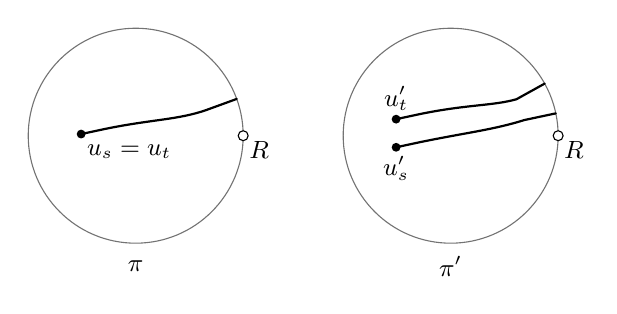
\begin{tikzpicture}[x=1.05cm,y=1.05cm,line cap=round,line join=round,
                    every node/.style={font=\small}]
  \begin{scope}
    \draw[black!55] (0,0) circle (1.30);
    \draw[thick] (-.66,.02) -- (-.38,.08)
       .. controls (.20,.20) and (.51,.19) .. (20:.91) -- (20:1.30);
    \fill (-.66,.02) circle (1.6pt);
    \node[below right,inner sep=2pt] at (-.66,-.04) {$u_s=u_t$};
    \filldraw[fill=white] (1.30,0) circle (1.8pt);
    \node[below right,inner sep=2pt] at (1.30,0) {$R$};
    \node at (0,-1.58) {$\pi$};
  \end{scope}
  \begin{scope}[xshift=4cm]
    \draw[black!55] (0,0) circle (1.30);
    \draw[thick] (-.66,.20) -- (-.38,.26)
       .. controls (.20,.38) and (.51,.36) .. (29:.91) -- (29:1.30);
    \fill (-.66,.20) circle (1.6pt);
    \node[above,inner sep=2pt] at (-.66,.23) {$u'_t$};
    \draw[thick] (-.66,-.14) -- (-.38,-.08)
       .. controls (.20,.04) and (.51,.07) .. (12:.91) -- (12:1.30);
    \fill (-.66,-.14) circle (1.6pt);
    \node[below,inner sep=2pt] at (-.66,-.17) {$u'_s$};
    \filldraw[fill=white] (1.30,0) circle (1.8pt);
    \node[below right,inner sep=2pt] at (1.30,0) {$R$};
    \node at (0,-1.58) {$\pi'$};
  \end{scope}
\end{tikzpicture}
\caption{Images of two disjoint vanishing disks in the base. Under $\pi$ the disks follow one path from their common critical value. Under $\pi'$ the same disks follow separate paths, in either prescribed order. The open circle marks the value of the reference fibre.}\label{fig:commonpaths}
\end{figure}
